%OOPS - the conversion from gamma relating P and rho to gamma relating T and P assumed rho proportional to P/T, which isn't correct for a variable mean molecular weight.
%Too late to fix for the assignment, but could be fixed for next year.

\documentclass[12pt]{article}
\usepackage{geometry}
\usepackage{hyperref}
\usepackage{amsmath}
\usepackage{graphicx}
\geometry{a4paper,tmargin=1.0cm,bmargin=2cm,lmargin=2cm,rmargin=2cm}
\begin{document}
\title{Description and Manual for {\tt star}}
\author{Prof Mike Ireland}
\maketitle

\section{A Personal Introduction}

The first time I taught a course on stellar physics was in 2009 at the University of Sydney.  I recalled being especially dissapointed as an undergraduate at not really understanding how {\em real} stars worked, and found polytropic examples not very instructive, as they averaged over a lot of physics but also were slightly too complex to develop a deep intuitive understanding. Cox and Giuli's Principles of Stellar Structure was a 700 page tome (2004 Weiss et al. edition) which was terse in places despite its length, and I believed there had to be a simpler way to both understand how stars work and end up with a result that matched real stars, including the sun. 

As the students were familiar with MATLAB, in one lecture I showed how we could solve the equations of stellar structure for the sun using Euler's method, while burying a lot of details in the opacity $\kappa$ (tabulated), the equation of state and adiabatic $\gamma$ (derived using the Saha equation via a mediocre set of comments), and the nuclear $\epsilon$ (taken I believe from publicly available Los Alamos tables).  The issues with this approach were that the model did not match the sun without adding mixing length theory, which was highly unsatisfactory as it defeated the purpose of making the code in the first place, and once a model was dominated by radiation at e.g. 2 M$_\odot$, using a shooting initial value problem method was inadequate as changes at the numerical precision in the core made large surface changes. 

When teaching my first 2nd year course (ASTR2013) at the Australian National University in 2019, I decided to re-do and hopefully simplify this code in python. The model I attempted to use was a star on the Hayashi track, which avoided the need to solve for the central density and temperature - one could simply set these and have a valid model of a cooling pre-main sequence star, as long as the central values were within the correct range. However, this was not as simple as hoped, with the series of approximation for a star with 4\,MK internal temperature displayed in Figure~\ref{figApprox}. There is relatively little difference between the models in the deep interior, with even the simplified ideal gas equation of state applying down to temperatures of $\sim 10^5$\,K. However, details really matter in the near-surface layers, and the cooling rate of this kind of star is highly dependent on the complex physics in these layers. The ``mixing-length'' theory in this model was at least understandable, as a linear interpolation between the adiabatic and radiative temperature gradients, according to what fraction of the luminosity could be carried by the internal energy of the gas moving at the sound speed.

\begin{figure}[h]
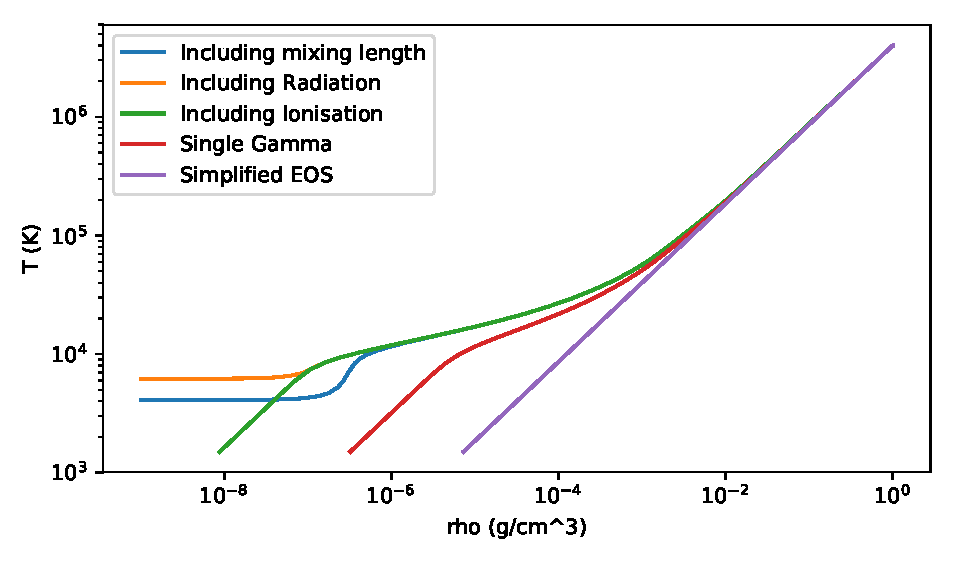
\includegraphics[width=0.75\textwidth]{ConvectiveStarApprox.pdf}
\caption{Temperature versus density throughout the convective star for the simplified and problem set "non-simplified" versions of the equation of state (purple and red lines), and additional approximations of increasing sophistication. The green line uses more than one $\gamma$ (called $\Gamma_1$, $\Gamma_2$ and $\Gamma_3$ in many older papers and texts), due to the ideal gas law no longer applying as the mean molecular weight changes during ionisation of H and He. The orange line explicitly changes the temperature gradient when the star becomes stable to radiation ($|dT/dr|_\text{rad} < |dT/dr|_\text{conv}$). The blue line gradually turns convection off (similar to `mixing length theory') when convection is unable to carry the stars luminosity, due to the low density, sound speed and internal energy per gram of the cool gas in the outer layers.}
\label{figApprox}
\end{figure}

After giving up on this complexity in 2020, where the only interior model we used in ASTR2013 was a white dwarf, in 2021 I returned to the problem of a simple stellar model from a different perspective. I realised that all the complexity of the fully convective star was in the surface layers (within 2\% of the stellar radius) and even with highly detailed mixing length theory, a free parameter would remain. So an interior model could still answer the question about the radius of a fully convective M dwarf given its measured effective temperature. A very simple ideal gas equation code was used, and this is the starting point for this model series, with only very small modifications.

A student of stellar interiors, with pre-requisites of 2nd year undergraduate physics and mathematics should be able to follow the gradually increasing complexity in these models in the following way:

\begin{enumerate}
\item In the beginning, we use only 2 equations of stellar structure and the ideal gas equation for the equation of state, plus a Gammow energy formulation of the nuclear energy created. For a given effective temperature or effective temperature-mass relation, this enables the mass-radius relation for very low mass stars to be derived.
\item We solve the Saha equation and create a tabulated equation of state, including the introduction of $\Gamma_1$, $\Gamma_2$ and $\Gamma_3$ as needed for phase transitions, which involves only a small extension to typical 2nd year undergraduate thermodynamics knowledge. 
\item Next, we add a surface condition evaluated an an optical depth beyond where mixing length theory is important, ideally from $<$3D$>$ atmospheres, or from deep atmospheres with a calibrated mixing length otherwise. This enables fully convective models to be created that are either in the process of cooling onto the main sequence, or evaluating equilibrium models on the lower main sequence. 
\item To extend further up the main sequence, we only now move to 4 equations of stellar structure, including radiative zones.
\item Enable the Hydrogen fraction $X$ to be time and spatially-variable, so that the evolution of the star can be traced through to the helium flash, and again to the first thermal pulse on the asymptotic giant branch.
\end{enumerate}

\section{Fully Convective Equations of Stellar Structure}

We begin with the two most fundamental equations of stellar structure, deriving from the conservation of mass and momentum. They are:

\begin{align}
\frac{dM}{dr} &= 4 \pi \rho(r) r^2 dr \\
\frac{dP}{dr} &= \frac{-GM(r)\rho(r)}{r^2} 
\end{align}

In addition, we define:

\begin{align}
\Gamma_1 &= \left( \frac{\partial \ln P}{\partial \ln \rho}\right)_S ,
\end{align}

noting that the adiabatic $\gamma=\Gamma_1$ in the case of pressure being dominated by gas pressure and no phase change (CITE Stothers02).  We set $S$ to be the total entropy and $s$ as the specific entropy in units of $k_B$ per baryon (useful later as baryon number is preserved, while the number of nucleii is not). It is now trivial to show that we can convert the second equation of stellar structure to:

\begin{align}
\frac{d \log_{10} \rho}{dr} &= - \frac{\rho \log_{10}e}{P(\rho, s) \Gamma_1 (\rho, s)} \frac{GM(r)}{r^2}.
\end{align}

In a first approximation, we will approximate $\Gamma_1 = \gamma = 5/3$, and use the ideal gas law:

\begin{align}
P = \frac{\rho}{u \mu} k_B T,
\end{align}

with a fixed value of $\mu=0.62$. We use the Sackur-Tetrode equation for entropy per baryon, which is complex to calculate for a particle mixture of species $i$ with de Broglie wavelengths $\Lambda_i(T)$:

\begin{align}
\frac{S}{k_B N_b} &=  \sum_i \frac{N_i}{N_b} \left[ \ln \left( \frac{V}{N_i \Lambda_i^3} \right) + \ln(g_i)\right]+ \frac{5}{2} \sum_i \left( \frac{N_i}{N_b} \right),
\end{align}

but follows the standard relationship for a gas of constant composition:

\begin{align}
P &= K(s) \rho^{5/3}
\end{align}

We will also approximate the Hydrogen burning nuclear luminostiy as:

\begin{align}
\epsilon(\rho, T) &= 2.52\times 10^6 X_1^2 \rho_\text{cgs} T_6^{-2/3} \exp(-33.8 T_6^{-1/3}) \text{\,erg\,s}^{-1}\text{g}^{-1},
\end{align}

where $T_6$ is the temperature in MK, and $\rho_\text{cgs}$ is the density in g\,cm$^{-3}$, and the hydrogen fraction $X_1=0.74$ for a zero age main sequence star. With this input physics, is it possible to answer the following questions:

\begin{enumerate}
\item For a central density of 100\,g\,cm$^{-3}$ and a central temperature of 8\,MK, find the mass and luminosity of the model.

\item Solve for the total mass, and compute a model with total mass 0.28\,M$_\odot$.

%dd = Table.read('EEM_dwarf_UBVIJHK_colors_Teff.txt', format='ascii.fixed_width')
\item Assuming an empirical solar-metalicity Mass-Teff relationship $T_\text{eff} = 2700 + 2000(M/M_\odot)$\,K, compute a mass radius relationship between 0.1 and 0.4\,$M_\odot$. Repeat this for a metal poor relationship $T_\text{eff} = 3000 + 2000(M/M_\odot)$\,K.
\end{enumerate}

\section{Adding an Equation of State}

The equation of state can be derived from chemical equilibrium equations, especially with regards to ions. The most important equation here is the Saha equation:

\begin{align}
n_{i+1} &= \frac{n_i}{n_e} \frac{2}{\lambda_e(T)^3} \frac{z_{i+1}(T)}{z_i(T)} \exp \left[ - \frac{(\epsilon_{i+1} - \epsilon_i)}{k_B T} \right],
\end{align}

where $z_i$ is the internal partition function for an atom of ionization state $i$ (often just the electronic spin degeneracy of the ground state), $\lambda_e(T)$ is the de~Broglie wavelength of the electron and $\epsilon_i$ is the $i$th ionisation energy of the atom. Phrasing the equation in this way makes it clear that at fixed $n_e$ and $T$, this is a linear equation in the $n_i$, resulting in a simple linear equation.

At lower temperatures, molecules complicate the picture, as all atoms are coupled together.  In this case, the Gibbs free energy of the system has to be minimised e.g. by the technique of Lagrange multipliers, as described in Sharp and Huebner (1990) or Tsuji (1973), with the original formulation of Russell (1934) the one we use here with $\log$ being $\log_{10}$:

\begin{align}
P_A P_B &= K_{AB}(T)P_{AB}\\
\log(P_A) + \log(P_B) - \log(P_{AB})&= \log(K_{AB}(T))\\
\rho &= \frac{m_H(P_H + P_{H+} + 2P_{H_2})}{X k_B T}\\
P_H + P_{H+} + 2P_{H_2} &= \frac{\rho X k_B T}{m_H}\\
\sum_i k P_{(A_i)_k} &= \frac{\rho f_A k_B T}{m_A}\\
&= \frac{\rho \epsilon_A k_B T}{\sum \epsilon_i m_i},
\end{align}

where $f_i$ is the mass fraction of element $i$ and $\epsilon_i$ is the number fraction of element $i$. We now re-phrase the Saha equation as the same form as Russell (1934) noting that the partial pressure of electrons, $P_e = n_e k_B T$ at the low pressures in stellar atmospheres, giving:

\begin{align}
P_{A+}P_e &= \left( \frac{2 k_B T}{\lambda_e(T)^3} \frac{z_{i+1}(T)}{z_i(T)} \exp \left[  \frac{-E_{A \rightarrow A+}}{k_B T} \right] \right) P_A \\
\log(P_{A+}) + \log(P_e) - \log(P_A) &= \log\left( \frac{2 k_B T}{\lambda_e(T)^3} \frac{z_{i+1}(T)}{z_i(T)} \right) - \frac{\log(e) E_{A \rightarrow A+}}{k_B T} ,
\end{align}

which enables us to identify the ionization equilibrium constant $K_A'$. We also have the equation for the electron partial pressure:

\begin{align}
\sum_i P_{A+_i}  - P_e &= 0.
\end{align}

For $m$ atoms, this gives 1 equation for $P_e$, $m$ linear equations in $P_A$ for each atom, $m$ logarithmic equations for each ion, and one equation for each molecular species. 

The end result of this are tables for $\Gamma_1$ and $P$, and a function that reads from them.

\section{Adding a Surface Condition from Photosphere and Upper Atmosphere Models}

The near surface conditions for a convective star is highly affected by inefficient convection, which is typically modelled by a mixing-length convection theory. The importance of the details of such a theory can be considered roughly as the ratio of the convective flux at $\tau=1$ to the radiative flux, i.e.:

\begin{align}
\frac{F_\text{conv, max}}{F_\text{rad}} &= \frac{g}{\kappa} \sqrt{\frac{k_B T}{u \mu}}  / \sigma_\text{SB} T^4 \\
&= \frac{k_B^{1/2}}{\sigma_\text{SB} u^{1/2}} \frac{g}{\kappa T^{3.5}}
\end{align}

For an M dwarf, with T$\sim$3500\,K, g$\sim10^{5}$\,cm\,s$^{-2}$ and $\kappa \sim 10^{-3}$\,cm$^2$\,g$^{-1}$, this ratio is $\sim$6000, meaning that mixing length shouldn't affect models significantly. However, for an M giant, this is much more significant, with the ratio being less than 1. For a solar type star, the value is approximately 100, meaning that convection can easily carry the flux, but requires velocities approximately 10\% of the sound speed and temperature contrasts of order 10\% of T$_\text{eff}$. For a late A star, this quantity is 0.1, meaning that convection effectively fails to transport flux.

For this reason, we will use the 3D Stagger grid within its region of validity, and Phoenix or MARCS models outside this, calibrated where possible to the edges of the Stagger grid. Both the $\sim$7000\,K warm edge of the models and the log($g$)=1.5 giant boundary of the models are expected to be poorly described by one-dimensional models incorporating mixing length theory, given the large anticipated temperature contrasts.

This new physics enables a number of real world problems:

\begin{enumerate}
\item Immediately, we can now compute the Zero Age Main Sequence (ZAMS) from a (formal) mass of 0.07\,M$_\odot$ to a mass of 0.3\,M$_\odot$, as a function of metallicity. The 0.07\,M$_\odot$ models are not realistic, because it takes more than the age of the universe to cool to this ZAMS model. This includes a minimum value of core entropy. 
\item For each mass and metallicity, we can now create an increasing entropy sequence from these ZAMS models. Each entropy will have a total internal (thermal plus gravitational) energy, and a difference between surface and interior luminosity. These form points on a differential equation, $dU/dt = L(t)$. In the simplest approximation, we can approximate $L$ as linearly varying in time, enabling a trapezoidal rule integration and $\Delta t = 2(U_1 - U_2)/(L_1 + L_2)$. Cooling tracks can then be directly compared to Baraffe et al. (2015 or 1998) tracks.
\end{enumerate}

\section{The Remaining Two Structure Equations}

Already, we have demonstrated that relatively simple physics combined with some tabulated atmospheric boundary conditions can reproduce some modern theoretical predictions. However, we are not yet up to understanding the structure or evolution of the sun.

\end{document}
